% Figure 1: Spatial mapping of Barrett reduction onto the 4x4 CGRA
\begin{figure}[hbt]
\centering
    \subfloat[Partial-product diagonals\label{fig:mapping:products}]{%
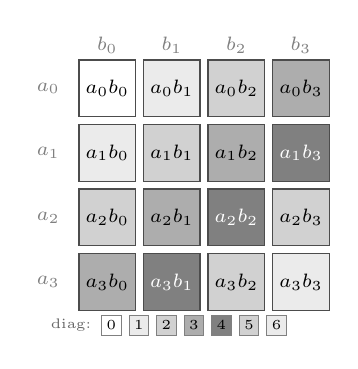
\begin{tikzpicture}[
  pe/.style={draw=black!70, line width=0.5pt, rectangle,
             minimum width=7.2mm, minimum height=7.2mm,
             font=\scriptsize, inner sep=0pt,
             outer sep=0pt, anchor=center},
  d0/.style={pe, fill=white},
  d1/.style={pe, fill=black!8},
  d2/.style={pe, fill=black!18},
  d3/.style={pe, fill=black!32},
  d4/.style={pe, fill=black!50, text=white},
  d5/.style={pe, fill=black!18},
  d6/.style={pe, fill=black!8},
  lbl/.style={font=\scriptsize, text=black!50},
]
\def\sp{0.82}  % spacing
% Column labels
\foreach \c/\lab in {0/$b_0$, 1/$b_1$, 2/$b_2$, 3/$b_3$}
  \node[lbl] at (\c*\sp, 0.55) {\lab};
% Row labels
\foreach \r/\lab in {0/$a_0$, 1/$a_1$, 2/$a_2$, 3/$a_3$}
  \node[lbl, anchor=east] at (-0.48, -\r*\sp) {\lab};
% Grid nodes
\node[d0] at (0*\sp, -0*\sp) {$a_0 b_0$};
\node[d1] at (1*\sp, -0*\sp) {$a_0 b_1$};
\node[d2] at (2*\sp, -0*\sp) {$a_0 b_2$};
\node[d3] at (3*\sp, -0*\sp) {$a_0 b_3$};
\node[d1] at (0*\sp, -1*\sp) {$a_1 b_0$};
\node[d2] at (1*\sp, -1*\sp) {$a_1 b_1$};
\node[d3] at (2*\sp, -1*\sp) {$a_1 b_2$};
\node[d4] at (3*\sp, -1*\sp) {$a_1 b_3$};
\node[d2] at (0*\sp, -2*\sp) {$a_2 b_0$};
\node[d3] at (1*\sp, -2*\sp) {$a_2 b_1$};
\node[d4] at (2*\sp, -2*\sp) {$a_2 b_2$};
\node[d5] at (3*\sp, -2*\sp) {$a_2 b_3$};
\node[d3] at (0*\sp, -3*\sp) {$a_3 b_0$};
\node[d4] at (1*\sp, -3*\sp) {$a_3 b_1$};
\node[d5] at (2*\sp, -3*\sp) {$a_3 b_2$};
\node[d6] at (3*\sp, -3*\sp) {$a_3 b_3$};
% Legend
\def\ly{-3*\sp - 0.55}
\node[font=\tiny, anchor=east, text=black!60] at (-0.08, \ly) {diag:};
\foreach \i/\sh in {0/0, 1/8, 2/18, 3/32, 4/50, 5/18, 6/8} {
  \pgfmathsetmacro{\lx}{\i*0.35 + 0.05}
  \node[fill=black!\sh, draw=black!50, line width=0.3pt,
        minimum size=2.5mm, inner sep=0pt, font=\tiny] at (\lx, \ly) {\i};
}
\end{tikzpicture}%
}%
\hfill
\subfloat[Barrett carry chain\label{fig:mapping:carry}]{%
\centering
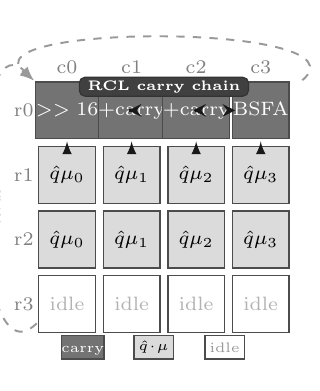
\begin{tikzpicture}[
  pe/.style={draw=black!70, line width=0.5pt, rectangle,
             minimum width=7.2mm, minimum height=7.2mm,
             font=\scriptsize, inner sep=0pt,
             outer sep=0pt, anchor=center},
  act/.style={pe, fill=black!55, text=white,
             text height=1.2ex, text depth=0.3ex},
  mid/.style={pe, fill=black!14},
  idl/.style={pe, fill=white, text=black!30},
  carry/.style={->, >=stealth, line width=1.0pt, black!90,
               shorten <=5pt, shorten >=5pt},
  dataup/.style={->, >=latex, line width=0.6pt, black!90,
                 shorten <=1pt, shorten >=1pt},
  wrap/.style={->, >=latex, dashed, line width=0.7pt, black!40,
               shorten <=1pt, shorten >=1pt},
  lbl/.style={font=\scriptsize, text=black!50},
  badge/.style={draw=black!80, fill=black!75, rounded corners=2pt,
                inner xsep=3pt, inner ysep=1.2pt,
                font=\tiny\bfseries, text=white},
]
\def\sp{0.82}  % spacing (same as subfig a)
% Fix bounding box to grid area (torus curves draw outside without affecting layout)
\useasboundingbox (-0.50, -3*\sp - 0.75) rectangle (3*\sp + 0.40, 1.05);
% Column labels
\foreach \c in {0,...,3}
  \node[lbl] at (\c*\sp, 0.55) {c\c};
% Row labels
\foreach \r in {0,...,3}
  \node[lbl, anchor=east] at (-0.30, -\r*\sp) {r\r};
% Row 0 — carry chain
\node[act] (c00) at (0*\sp, 0) {$>>16$};
\node[act] (c01) at (1*\sp, 0) {+carry};
\node[act] (c02) at (2*\sp, 0) {+carry};
\node[act] (c03) at (3*\sp, 0) {BSFA};
% Row 1
\node[mid] (c10) at (0*\sp,-1*\sp) {$\hat{q}\mu_0$};
\node[mid] (c11) at (1*\sp,-1*\sp) {$\hat{q}\mu_1$};
\node[mid] (c12) at (2*\sp,-1*\sp) {$\hat{q}\mu_2$};
\node[mid] (c13) at (3*\sp,-1*\sp) {$\hat{q}\mu_3$};
% Row 2
\node[mid] (c20) at (0*\sp,-2*\sp) {$\hat{q}\mu_0$};
\node[mid] (c21) at (1*\sp,-2*\sp) {$\hat{q}\mu_1$};
\node[mid] (c22) at (2*\sp,-2*\sp) {$\hat{q}\mu_2$};
\node[mid] (c23) at (3*\sp,-2*\sp) {$\hat{q}\mu_3$};
% Row 3
\node[idl] (c30) at (0*\sp,-3*\sp) {idle};
\node[idl] (c31) at (1*\sp,-3*\sp) {idle};
\node[idl] (c32) at (2*\sp,-3*\sp) {idle};
\node[idl] (c33) at (3*\sp,-3*\sp) {idle};
% RCL badge above row 0
\node[badge] at (1.5*\sp, 0.30) {RCL carry chain};
% Carry chain arrows
\draw[carry] ([xshift=6pt]c00.east) -- ([xshift=6pt]c01.west);
\draw[carry] ([xshift=6pt]c01.east) -- ([xshift=6pt]c02.west);
\draw[carry] ([xshift=6pt]c02.east) -- ([xshift=6pt]c03.west);
% Vertical arrows (rows 1→0)
\foreach \c in {0,...,3}
  \draw[dataup] (c1\c.north) -- (c0\c.south);
% Torus col wrap: c3→c0 (curve above column labels)
\draw[wrap] ([xshift=4pt]c03.north east)
  .. controls +(0.9, 0.75) and +(-0.9, 0.75) ..
  (c00.north west);
% Torus row wrap: r3→r0 (curve left of row labels)
\draw[wrap] ([yshift=4pt]c30.south west)
  .. controls +(-0.9, -0.9) and +(-0.9, 0.9) ..
  (c00.north west);
\node[font=\tiny\itshape, text=black!40, rotate=90]
  at (-0.9, -1.5*\sp) {torus};
% Legend
\def\ly{-3*\sp - 0.55}
\node[act, minimum width=5mm, minimum height=3mm, font=\tiny] at (0.2, \ly) {carry};
\node[mid, minimum width=5mm, minimum height=3mm, font=\tiny] at (1.1, \ly) {$\hat{q}\!\cdot\!\mu$};
\node[idl, minimum width=5mm, minimum height=3mm, font=\tiny,
      text=black!40] at (2.0, \ly) {idle};
\end{tikzpicture}%
}%
\caption{Spatial mapping of Barrett reduction onto the 4$\times$4 CGRA.
(a)~PE$(r,c)$ computes $a_r \cdot b_c$; shading marks partial-product diagonals ($k{=}r{+}c$), not communication hops.
(b)~Row~0 implements the RCL carry chain, while dashed torus links bound quotient/carry travel to at most 4 hops.}

\label{fig:mapping}
\end{figure}